%-----------------------------------------------------------------------------------------------------------------------------------------------%
%	The MIT License (MIT)
%
%	Copyright (c) 2015 Jan Küster
%
%	Permission is hereby granted, free of charge, to any person obtaining a copy
%	of this software and associated documentation files (the "Software"), to deal
%	in the Software without restriction, including without limitation the rights
%	to use, copy, modify, merge, publish, distribute, sublicense, and/or sell
%	copies of the Software, and to permit persons to whom the Software is
%	furnished to do so, subject to the following conditions:
%
%	THE SOFTWARE IS PROVIDED "AS IS", WITHOUT WARRANTY OF ANY KIND, EXPRESS OR
%	IMPLIED, INCLUDING BUT NOT LIMITED TO THE WARRANTIES OF MERCHANTABILITY,
%	FITNESS FOR A PARTICULAR PURPOSE AND NONINFRINGEMENT. IN NO EVENT SHALL THE
%	AUTHORS OR COPYRIGHT HOLDERS BE LIABLE FOR ANY CLAIM, DAMAGES OR OTHER
%	LIABILITY, WHETHER IN AN ACTION OF CONTRACT, TORT OR OTHERWISE, ARISING FROM,
%	OUT OF OR IN CONNECTION WITH THE SOFTWARE OR THE USE OR OTHER DEALINGS IN
%	THE SOFTWARE.
%
%
%-----------------------------------------------------------------------------------------------------------------------------------------------%

%============================================================================%
%	DOCUMENT DEFINITION
%============================================================================%

%we use article class because we want to fully customize the page and dont use a cv template
\documentclass[10pt,A4]{article}



%	ENCODING

%we use utf8 since we want to build from any machine
\usepackage[utf8]{inputenc}



%	LOGIC

% provides \isempty test
\usepackage{xifthen}



%	FONT

% some tex-live fonts - choose your own

%\usepackage[defaultsans]{droidsans}
%\usepackage[default]{comfortaa}
%\usepackage{cmbright}
%\usepackage[default]{raleway}
%\usepackage{fetamont}
%\usepackage[default]{gillius}
%\usepackage[light,math]{iwona}
\usepackage[thin]{roboto}

% set font default
\renewcommand*\familydefault{\sfdefault}
\usepackage[T1]{fontenc}

% more font size definitions
\usepackage{moresize}



%	PAGE LAYOUT  DEFINITIONS

%debug page outer frames
%\usepackage{showframe}

%define page styles using geometry
\usepackage[a4paper]{geometry}

% for example, change the margins to 2 inches all round
\geometry{top=1.75cm, bottom=-.6cm, left=1.5cm, right=1.5cm}

%use customized header
\usepackage{fancyhdr}
\pagestyle{fancy}

%less space between header and content
\setlength{\headheight}{-5pt}

%customize entries left, center and right
\lhead{}
\chead{
  \textcolor{txtcol}{\textbf{Consultant and Software Engineer}} \textcolor{sectcol}{$\oplus$}
  \textcolor{txtcol}{\textbf{Roanoke, Virgina}} \textcolor{sectcol}{$\oplus$}
  \textcolor{txtcol}{\textbf{dconner.pro@gmail.com}} \textcolor{sectcol}{$\oplus$}
  \textcolor{txtcol}{\textbf{+1 (540) 761-1257}}
}
\rhead{}

%indentation is zero
\setlength{\parindent}{0mm}

%	TABLE /ARRAY/LIST DEFINITIONS

%for layouting tables
\usepackage{multicol}
\usepackage{multirow}

%extended aligning of tabular cells
\usepackage{array}

\newcolumntype{x}[1]{%
>{\raggedleft\hspace{0pt}}p{#1}}%

\usepackage{enumitem}

%	GRAPHICS DEFINITIONS

%for header image
\usepackage{graphicx}

%for floating figures
\usepackage{wrapfig}
\usepackage{float}
%\floatstyle{boxed}
%\restylefloat{figure}

%for drawing graphics
\usepackage{tikz}
\usetikzlibrary{shapes, backgrounds,mindmap, trees}


%	Color DEFINITIONS

\usepackage{color}

%accent color
%\definecolor{bgcol}{RGB}{120,110,100}
\definecolor{bgcol}{RGB}{140,130,120}

%dark background color
%\definecolor{sectcol}{RGB}{204,110,0}
\definecolor{sectcol}{RGB}{30,25,18}

%light background / accent color
\definecolor{softcol}{RGB}{225,225,225}

%text color
%\definecolor{txtcol}{RGB}{60,50,45}
\definecolor{txtcol}{RGB}{25,20,15}


%============================================================================%
%	DEFINITIONS
%============================================================================%

% 	HEADER

% remove top header line
\renewcommand{\headrulewidth}{0pt}

%remove botttom header line
\renewcommand{\footrulewidth}{0pt}

%remove pagenum
\renewcommand{\thepage}{}

%remove section num
\renewcommand{\thesection}{}


% 	ARROW GRAPHICS in Tikz

% a six pointed arrow poiting to the left
\newcommand{\tzlarrow}{(0,0) -- (0.2,0) -- (0.3,0.2) -- (0.2,0.4) -- (0,0.4) -- (0.1,0.2) -- cycle;}

% include the left arrow into a tikz picture
% param1: fill color
%
\newcommand{\larrow}[1]
{\begin{tikzpicture}[scale=0.58]
	 \filldraw[fill=#1!100,draw=#1!100!black]  \tzlarrow
 \end{tikzpicture}
}

% a six pointed arrow poiting to the right
\newcommand{\tzrarrow}{ (0,0.2) -- (0.1,0) -- (0.3,0) -- (0.2,0.2) -- (0.3,0.4) -- (0.1,0.4) -- cycle;}

% include the right arrow into a tikz picture
% param1: fill color
%
\newcommand{\rarrow}
{
\begin{tikzpicture}[scale=0.7]
	\filldraw[fill=sectcol!100,draw=sectcol!100!black] \tzrarrow
 \end{tikzpicture}
}


%	custom sections


% create a coloured box with arrow and title as cv section headline
% param 1: section title
%
\newcommand{\cvsection}[1]
{
\colorbox{bgcol}{\makebox[1\linewidth][l]{
	\larrow{sectcol} \hspace{-8pt} \larrow{sectcol} \hspace{-8pt} \larrow{sectcol} \textcolor{white}{\textbf{#1}}\hspace{4pt}
}}
}

%create a coloured arrow with title as cv meta section section
% param 1: meta section title
%
\newcommand{\metasection}[2]{
	\begin{tabular*}{1\linewidth}{p{0.18\linewidth} p{0.76\linewidth}}
		\larrow{bgcol}\normalsize{\textbf{\textcolor{sectcol}{#1}}}&#2\\
	\end{tabular*}
}


%	 CV EVENT

% creates a stretched box as cv entry headline followed by two paragraphs about
% the work you did
% param 1:	event time i.e. 2014 or 2011-2014 etc.
% param 2:	event name (what did you do?)
% param 3:	institution (where did you work / study)
% param 4:	what was your position
% param 5:	some words about your contributions
%
\newcommand{\cvevent}[5] {
\begin{flushleft}
\small{\textcolor{txtcol}{#3}}\\
\small{\textbf{#1 \hfill #2}}\\[-7pt]
\textcolor{softcol}{\hrule}
\vspace{\spread}
\begin{tabular*}{1\linewidth}{p{0.001\linewidth} p{0.9\linewidth}}
	\larrow{bgcol} & #4 \\[2pt]
	\larrow{bgcol} & #5 \\[\spread]
\end{tabular*}
\end{flushleft}
%\textcolor{softcol}{\hrule}
}

% creates a stretched box as
\newcommand{\cveventmeta}[2] {
	\mbox{\mystrut \hspace{87pt}\textit{#1}}\\
	#2
}


% CUSTOM STRUT FOR EMPTY BOXES
%----------------------------------------- -----------------------------------------------
\newcommand{\mystrut}{\rule[-.3\baselineskip]{0pt}{\baselineskip}}


% CUSTOM LOREM IPSUM

\newcommand{\lorem}
{Lorem ipsum dolor sit amet, consectetur adipiscing elit. Donec a diam lectus.}


% SPREAD

\newcommand{\spread}{7pt}


\begin{document}

%use our custom fancy header definitions
\pagestyle{fancy}

\begin{minipage}[t]{0.485\textwidth}



\vspace{\spread}

%	TITLE HEADLINE
\hspace{-0.25\linewidth}\colorbox{bgcol}{\makebox[1.25\linewidth][c]{\textcolor{sectcol}{\rule[-1mm]{1mm}{1.0cm}} \HUGE{\textcolor{white}{\textsc{ David Conner}} } }}
%---------------------------------------------------------------------------------------
%	HEADER IMAGE
% \hspace{-0.25\linewidth}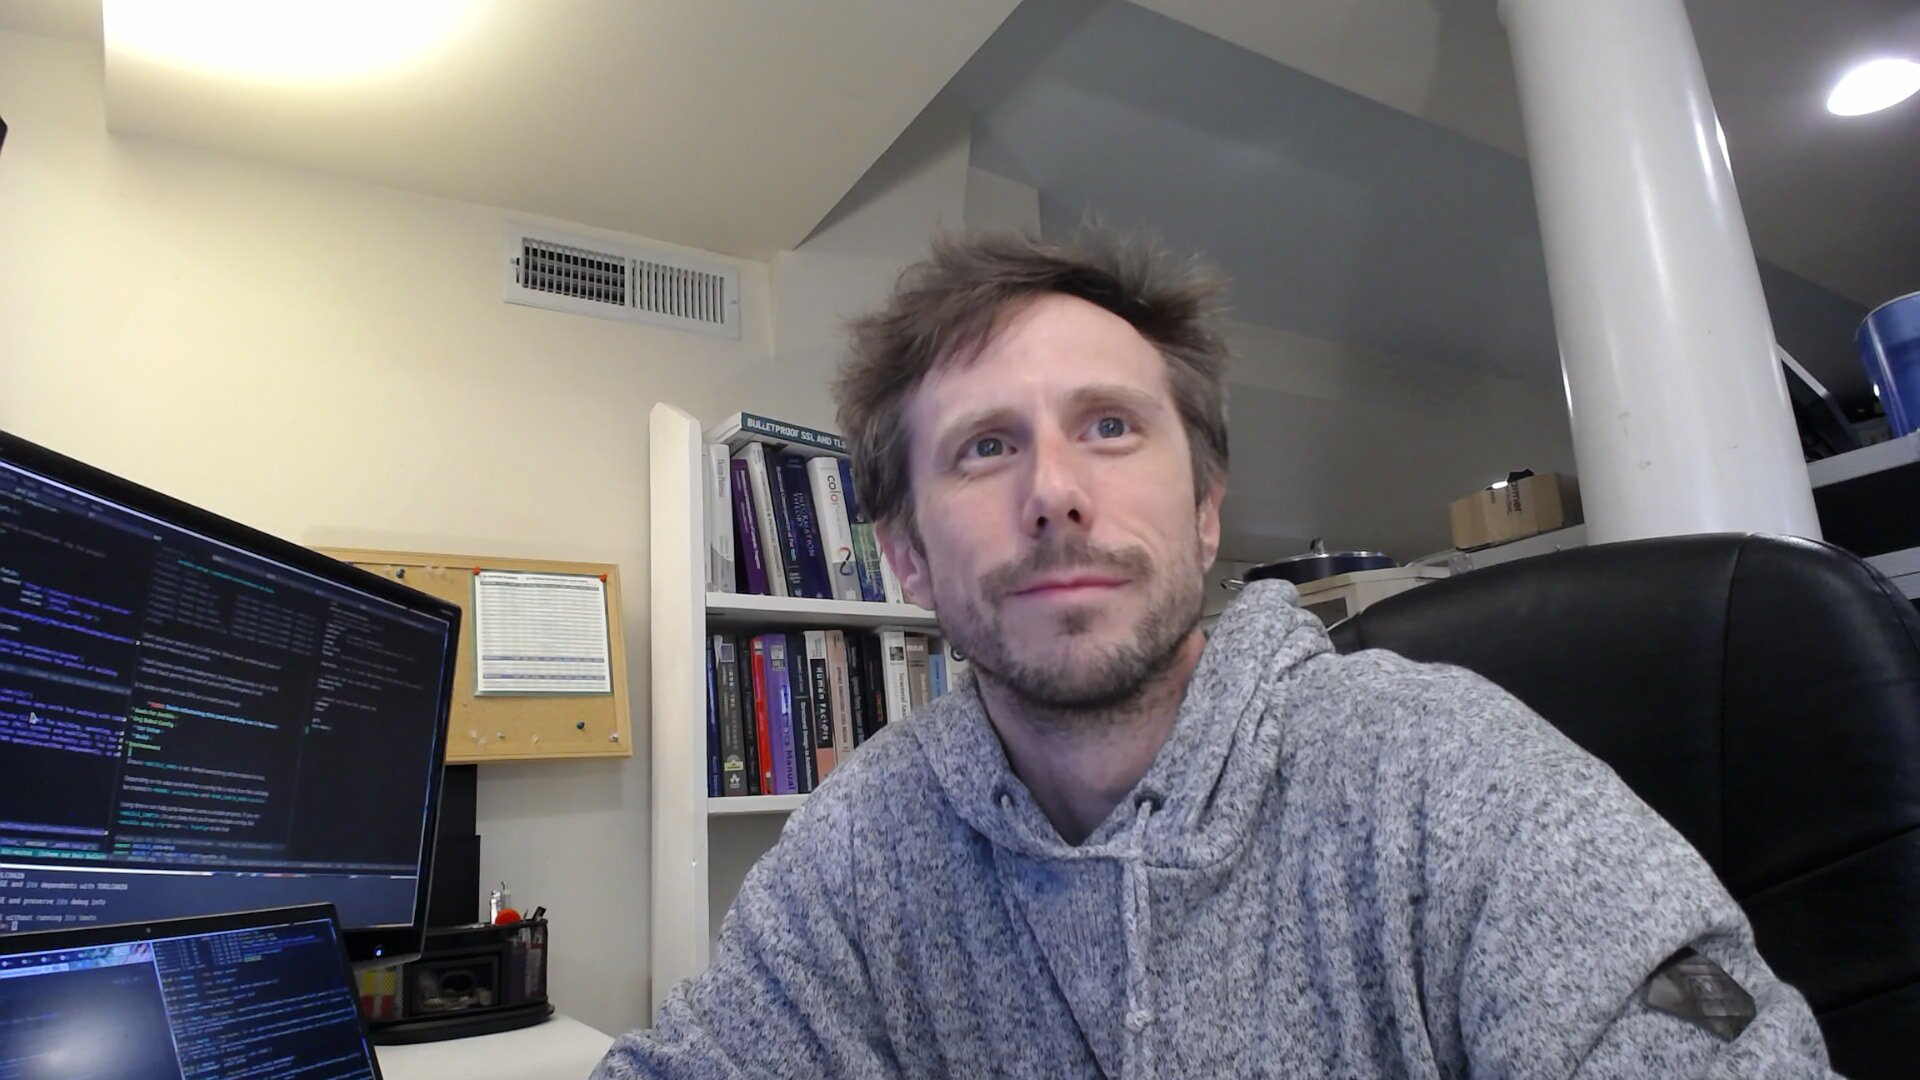
\includegraphics[width=1.2725\linewidth]{myphoto.jpg} %use full size
%---------------------------------------------------------------------------------------
%	QR CODE (optional)
%\vspace{-100pt}
%\hspace{0.59\linewidth}
%
\includegraphics[width=88pt]{qrcode}
%\normalsize
\vspace{-0.1cm}\\
%\cvsection{Summary}\\
\vspace{-0.1cm}\\
\color{black}I am a digital media graduate (M.Sc.) with project experience in educational
research as well as in the private sector. During my studies I focused on
e-assessment software and moved over to b2b software for IBM Notes Domino.

\end{minipage}
\hfill
\begin{minipage}[t]{0.485\textwidth}


%---------------------------------------------------------------------------------------
%	SUMMARY (optional)
\vspace{\spread}

\cvsection{Summary}\\
I am a digital media graduate (M.Sc.) with project experience in educational
research as well as in the private sector. During my studies I focused on
e-assessment software and moved over to b2b software for IBM Notes Domino.

Currently I develop and evaluate the next generation learning management system
with Meteor based on an extensive nursing curriculum for healthcare education.
I also love fitness, martial arts, videogames, news and Sci-Fi series.\\[-2pt]
\textcolor{softcol}{\hrule}

\end{minipage}

\begin{minipage}[t]{0.485\textwidth}

\vspace{\spread}

%---------------------------------------------------------------------------------------
%	META SECTION
\metasection{Status:}{Fullstack JS Engineer, M.Sc. Digital Media, Consultant}
\metasection{Fields:}{Project Management, Software Development, Consulting}
\end{minipage}
\hfill
\begin{minipage}[t]{0.485\textwidth}

\vspace{5pt}

\metasection{Tech:}{Meteor, Javascript, Bootstrap, Mongodb, Git, Webstorm, Sourcetree, Terminal}
\metasection{Loves:}{Global Game Jam, Sci-Fi series, Stackoverflow, Fitness and Martial Arts}
\end{minipage}

\begin{minipage}[t]{0.485\textwidth}

\vspace{\spread}



%---------------------------------------------------------------------------------------
%	EDUCATION SECTION

\cvsection{Education}\cvevent{2021 - 2023; 2006 - 2008}
{Mechatronics Systems E.T.}
{Virginia Western Community College}
{Master Thesis: Semi Automated Scoring in Technology Based Assessment}
{Developed and evaluated an algorithm for semi automated scoring of spreadsheet data}

%\textcolor{softcol}{\hrule}
\cvevent{2004-2006}
{Computer Science}
{Virginia Tech}
{Co-Invented a touch table application for medical support, co-developed software (Java) }
{Formed a scrum team, mainted project dev server (Debian), surveyed target audience}

%\textcolor{softcol}{\hrule}
\cvsection{Education}\cvevent{2012 - 2015}
{Master Studies Digital Media}
{University of Bremen}
{Inter-cultural classes in English, covering special topics in computer science and design}
{Professionalized in research methods, software development and e-assessment}

\cvevent{2009 - 2010}
{Semester Abroad}
{University of Melbourne}
{Mastered six months of study and trans-cultural experience in Melbourne, Australia}
{Finished machine programming, information visualization, professional essay writing}

\cvevent{2007 - 2012}
{Bachelor Studies Digital Media}
{University of Bremen}
{Fundamentals in Computer Science}
{Bachelor thesis focused on experimental redesign of the keyboard to support functional illiterates.}

%\textcolor{softcol}{\hrule}

\end{minipage}
\hfill
\begin{minipage}[t]{0.485\textwidth}

\vspace{\spread}



%---------------------------------------------------------------------------------------
%	EXPERIENCE

\cvsection{Experience}\cvevent{2022 - 2023}
{Engineering Student Aide}
{Virginia Western Community College}
{Maintain Ender-3 Pro and Raise3D printers. Synced Ender-3 configurations for PLA plastics}
{Created an Autodesk Fusion CNC config for a Velocity CNC. Collected notes on almost all equipment including support links and digital copies of manuals}

\cvevent{2018}
{Cloud Engineer}
{RAKE Digital}
{Used MS SQL table metadata to quickly learn the accounting database schema for Millennium and ReadyPay}
{Designed an application stack with LoopbackJS and Angular 6 to automate payroll tasks in Azure}

\cvevent{2015 - 2017}
{Founder}
{Voxxel (Startup)}
{Built a Rails API to back prototypes in iOS, Android and AngularJS (with Web Audio)}
{Voxxel enabled fans to score their impersionations of movie quotes and accents}

\cvevent{2011 - 2015}
{Founder}
{Oscil8 (Startup)}
{Oscil8 was designed to be the “Github for Music Producers”}
{Developed a business model and strategic vision}

\cvevent{2014}
{Student Assistant / Programmer}
{Left + Right (Contract)}
{Developed a web service to extend a Ruby on Rails application with reporting on SQL Views}
{Cached report results in MongoDB to enable a dashboard}

\cvevent{2013}
{Student Assistant / Programmer}
{Jumpcloud}
{Full stack development using a NodeJS API and MongoDB}
{Integration tests using Mocha, Selenium and Soda}

\end{minipage}


%	ARTIFICIAL FOOTER (fancy footer cannot exceed linewidth)

\null
\vspace*{\fill}
% this won't print
%\hspace{-0.25\linewidth}\colorbox{gray}{\makebox[1.5\linewidth][c]{\mystrut  \textcolor{bgcol}{www.jankuester.com $\cdot$ github.com/jankapunkt}}}
%\hspace{-0.25\linewidth}\colorbox{bgcol}{\makebox[1.5\linewidth][c]{\mystrut \textmd{\textcolor{white}{https://te.xel.io $\cdot$ github.com/dcunited001}}}}

\end{document}
